\chapter{Results and Conclusions}
In this section we will describe our results and any conclusions we may have drawn from them as well as decisions that came from these results.
\section{Convolutional Neural Networks: Results}
All the neural network here are conv nx3x3 - conv nx3x3 - max pool 2x2 no strides - conv nx3x3 - conv nx3x3 - max pool 2x2 no strides - Dense 256 - Dense 128 - Dense Softmax 10 with Relu activations in the rest of the layers. Where this is not true we will note as such
\subsection{Number of Filters}
For this we are evaluating the following models:
\begin{itemize}
	\item 8-8-14-14 with 3x3 filters
	\item 24-24-32-32 with 3x3 filters
	\item 32-32-64-64 with 3x3 filters
	\item 48-48-96-96 with 3x3 filters
	\item 128-128-256-256 with 3x3 filters
\end{itemize}
For the results we are presenting here we are using data augmentation in all cases to reduce overfitting as well as early stopping to get the best model possible from our training. We have results for both colour and black and white for this evaluation.

We will only be presenting the colour results in this part as we will be evaluating the impact of colour in a later part.

\subsubsection{Effects on Training Speed}
As we increase the amount of filters we see our training speed declining as the number of neurons increases, this makes sense as you increase the number of computations that need to be done each epoch somewhat.

We ommit actual data here we were unable to control running parameters exactly due to these tests having to be run over several nights at different system workloads which would affect the results but our observations showed that we can get a range of 12s per epoch on our smallest model to 57s per epoch on our most complicated model
\subsubsection{Effects on Performance}
We begin this investigation assuming we will get better results with more. 
\begin{figure}
	\begin{tabular}{cc}
		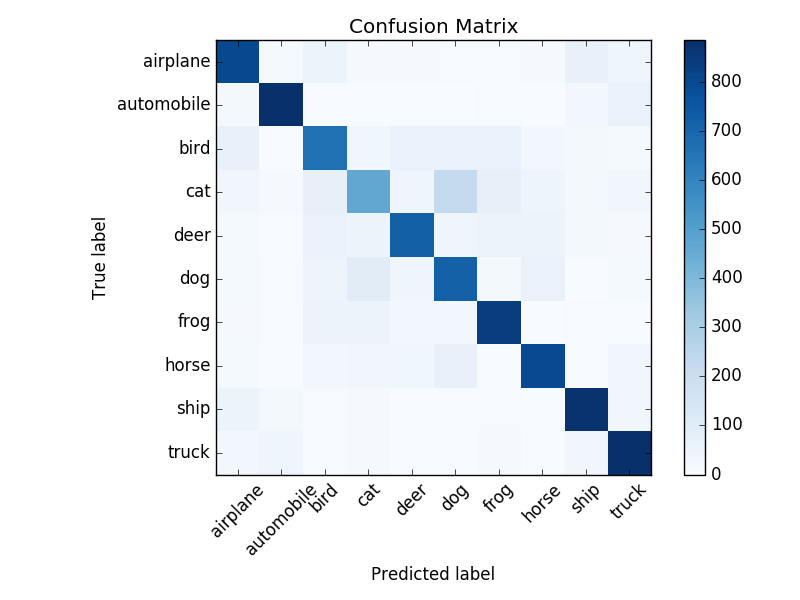
\includegraphics[width=0.45\linewidth]{8-8-14-14-3x3-15pct-color_confusion_matrix} &   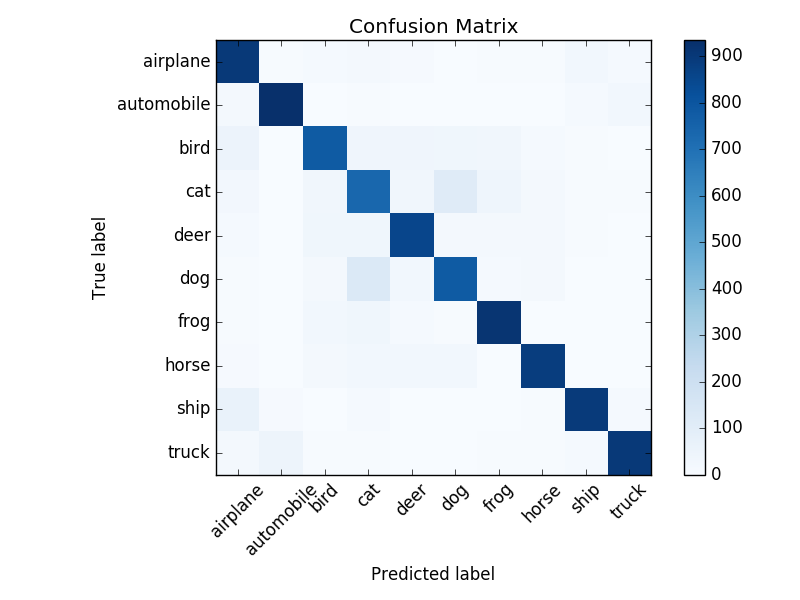
\includegraphics[width=0.45\linewidth]{24-24-48-48-3x3-15pct-color_confusion_matrix} \\
		(a) 8-8-14-14 & (b) 24-24-32-32 \\[6pt]
		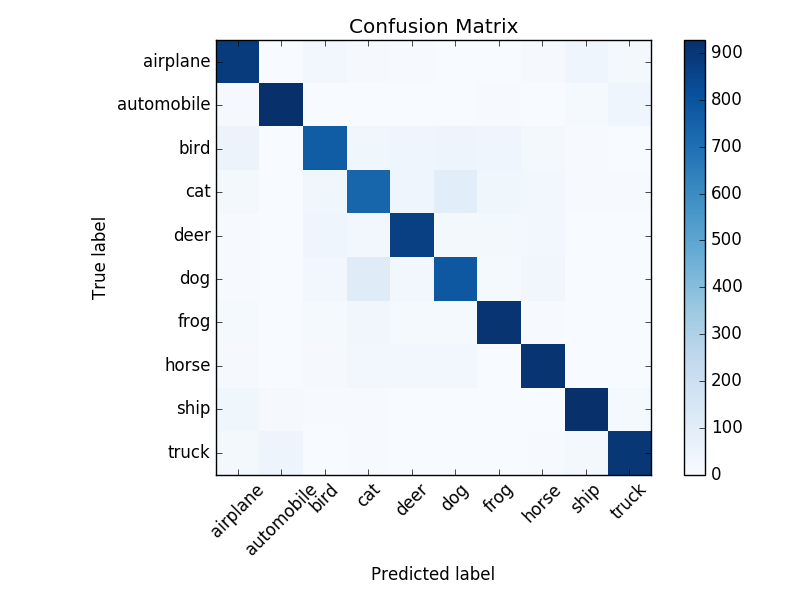
\includegraphics[width=0.45\linewidth]{32-32-64-64-3x3-15pct-color_confusion_matrix} &   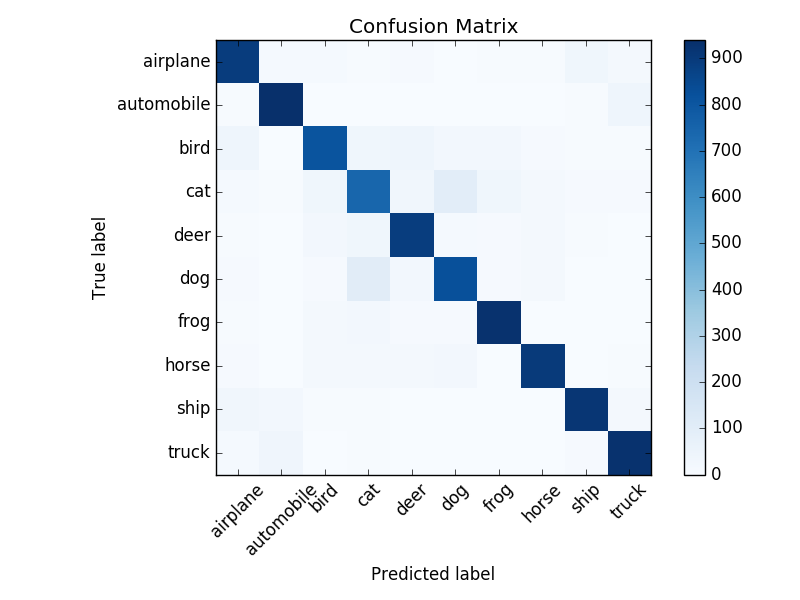
\includegraphics[width=0.45\linewidth]{48-48-96-96-3x3-15pct-color_confusion_matrix} \\
		(c) 32-32-64-64 & (d) 48-48-96-96 \\[6pt]
		\multicolumn{2}{c}{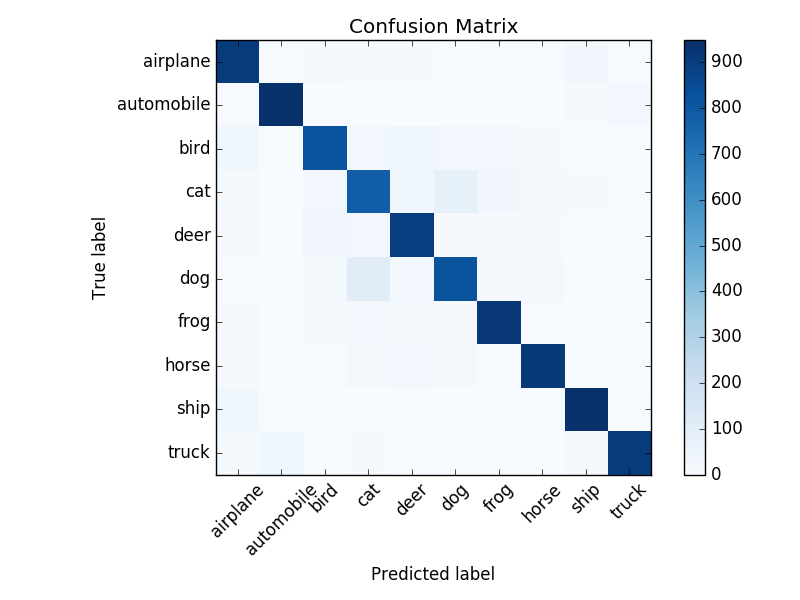
\includegraphics[width=0.45\linewidth]{128-128-256-256-3x3-15pct-no-strides-color_confusion_matrix} }\\
		\multicolumn{2}{c}{(e) 128-128-256-256}
	\end{tabular}
	\caption{Confusion Matrices varied by filter number}
\end{figure}

As we can see from the figures, a significant improvement between out smallest model and out largest one. However it appears we hit diminishing returns after a certain number of filters as we presumably hit the limit of the features we can draw from our small 32x32 data.

From the qualification report we also see an interesting pattern we hinted on earlier in this document. Dogs and Cats are the worst performing classes with confusing happening mostly between them but dogs get confused less with cats than the opposite.

This becomes clearer when we look at the classification reports.
\begin{figure}
\begin{verbatim}
8-8-14-14:
             precision    recall  f1-score   support
             
          0       0.78      0.72      0.75      1000
          1       0.84      0.90      0.87      1000
          2       0.67      0.55      0.61      1000
          3       0.55      0.45      0.50      1000
          4       0.64      0.72      0.68      1000
          5       0.63      0.65      0.64      1000
          6       0.73      0.83      0.77      1000
          7       0.74      0.81      0.77      1000
          8       0.80      0.84      0.82      1000
          9       0.86      0.82      0.84      1000
             
   avg / total       0.73      0.73      0.73     10000
\end{verbatim}
\begin{verbatim}  
24-24-48-48:
             precision    recall  f1-score   support
             
          0       0.82      0.90      0.86      1000
          1       0.93      0.94      0.93      1000
          2       0.84      0.78      0.81      1000
          3       0.71      0.74      0.72      1000
          4       0.85      0.86      0.86      1000
          5       0.79      0.78      0.79      1000
          6       0.88      0.91      0.90      1000
          7       0.91      0.89      0.90      1000
          8       0.93      0.90      0.91      1000
          9       0.94      0.90      0.92      1000
             
   avg / total       0.86      0.86      0.86     10000
\end{verbatim}
\begin{verbatim}    
32-32-64-64:
             precision    recall  f1-score   support
             
          0       0.84      0.89      0.86      1000
          1       0.94      0.93      0.93      1000
          2       0.83      0.77      0.80      1000
          3       0.74      0.74      0.74      1000
          4       0.85      0.87      0.86      1000
          5       0.80      0.79      0.79      1000
          6       0.89      0.91      0.90      1000
          7       0.89      0.91      0.90      1000
          8       0.91      0.93      0.92      1000
          9       0.92      0.90      0.91      1000
             
   avg / total       0.86      0.86      0.86     10000
\end{verbatim}
\begin{verbatim}  
48-48-96-96:  
             precision    recall  f1-score   support
             
          0       0.87      0.89      0.88      1000
          1       0.92      0.94      0.93      1000
          2       0.87      0.81      0.84      1000
          3       0.76      0.74      0.75      1000
          4       0.86      0.89      0.88      1000
          5       0.83      0.82      0.83      1000
          6       0.91      0.93      0.92      1000
          7       0.92      0.90      0.91      1000
          8       0.92      0.92      0.92      1000
          9       0.90      0.93      0.92      1000
             
    avg / total       0.88      0.88      0.88     10000
\end{verbatim}
\begin{verbatim}  
128-128-256-256:
             precision    recall  f1-score   support
             
          0       0.87      0.91      0.89      1000
          1       0.95      0.95      0.95      1000
          2       0.87      0.82      0.84      1000
          3       0.77      0.78      0.78      1000
          4       0.85      0.89      0.87      1000
          5       0.85      0.82      0.83      1000
          6       0.90      0.92      0.91      1000
          7       0.93      0.92      0.92      1000
          8       0.92      0.94      0.93      1000
          9       0.96      0.91      0.93      1000
             
   avg / total       0.89      0.89      0.88     10000
\end{verbatim}
\caption{Classification Reports for experiments}
\end{figure}

As you might notice from the figures above we stop seeing overall improvements at 48-48-96-96 with small improvement in some classes, but the extra cost of the larger networks makes it a good compromise for further experiments.
\subsubsection{Effects on Size of Weights}
This investigation is much simpler. We look at the sizes of the weights we store for each network and try to correlate it the number of calculations and network complexity.
\begin{figure}
	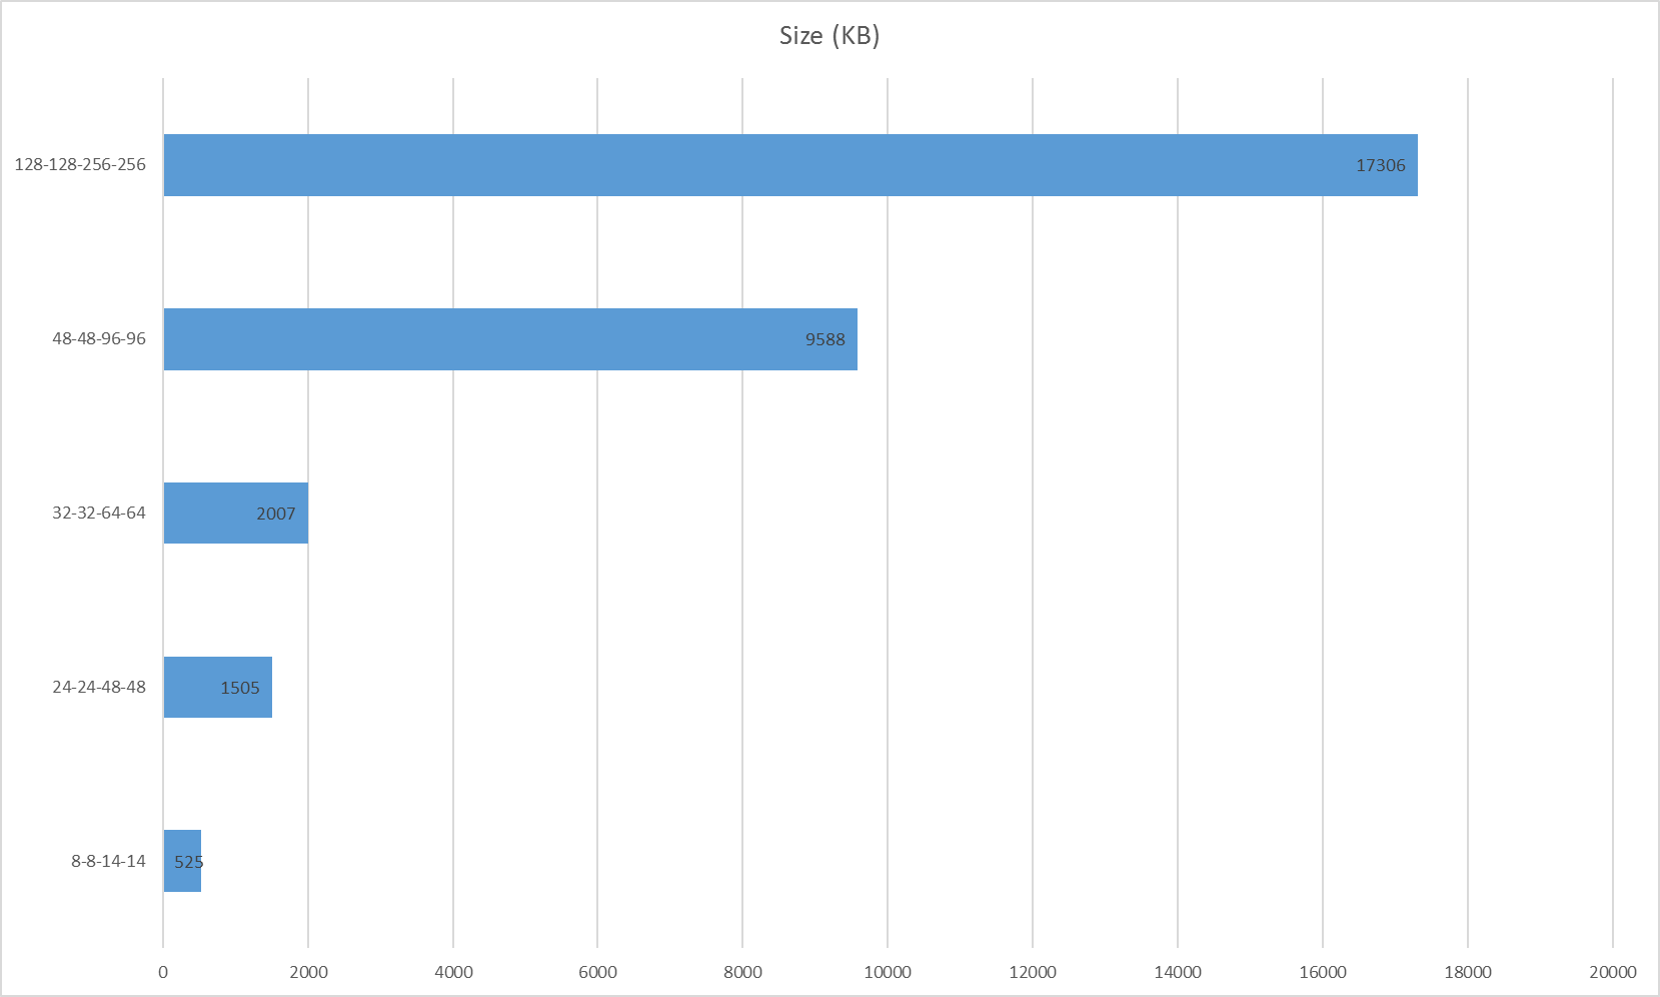
\includegraphics[width=0.8\linewidth]{datasizes_filters}
	\caption{Bar Chart of Size of Stored Weights}
\end{figure}

\subsection{Size of Filters}
\subsubsection{Effects on Training Speed}
\subsubsection{Effects on Performance}
\subsubsection{Effects on Size of Weights}

\subsection{Number of Colour Channels}
\subsubsection{Effects on Training Speed}
\subsubsection{Effects on Performance}
\subsubsection{Effects on Size of Weights}

\subsection{Number of Hidden Layers}
\subsubsection{Effects on Training Speed}
\subsubsection{Effects on Performance}
\subsubsection{Effects on Size of Weights}

\subsection{Augmentation}
\subsubsection{Effects on Training Speed}
\subsubsection{Effects on Overfitting}
\subsubsection{Effects on Performance}

\subsection{Multi Layer Perceptron: Figures in Matrices}

\section{Miscellaneous Discussion}
\subsection{Accounts of Early Experiments}
Here we will discuss the earliest parts of our experimentation. These were done before the experimental infastructure was complete so we don't have complete figures recorded for them. These accounts are based on logs and diary entries taken at the time. Rapid prototyping was taking place at the time so results might not be consistent. As a result this section is included in a pure discussion format and is aimed to offer some insight to early decisions taken in this project.

\subsubsection{Early Experiments}
